%! Author = Len Washington III
%! Date = 11/12/2023

% Preamble
\documentclass[25]{cs430lecture}
\usepackage{algpseudocode}

% Packages

% Document
\begin{document}

%<*Lecture-Activity-25>
\newcommand{\edges}[1]{\emph{\textbf{#1 edges\label{dfn:#1-edges}}}}%
\maketitle
\openingquestions

\begin{enumerate}
    \item What is the runtime of breadth first search
	(if you restart the search from a new source if everything was not visited from the first source)?
	\answer{$O(|V|+|E|)$.
	Use a queue for all vertices that haven't been visited.
	Keep track of $d$-distance to edges and $\pi$-precescessor of which edge got us there.}
	\item Does a breadth-first search always reach all vertices?
	\answer{No.}
	\item How can you use a breadth-first search to find the shortest path (minimum number of edges) from a given source vertex to all other vertices?
	\answer{Use the $d$ variable which holds the distance to edges from the source.}
	\item If you look at the predecessor edges which were used to connect to an unvisited vertex, what do these predecessor edges form?
	Is it unique for a graph?
	\answer{They yield a breadth-first tree.}
\end{enumerate}

\section{Depth-First Search}\label{sec:depth-first-search}
\url{https://www.reddit.com/r/dataisbeautiful/comments/7b7aa0/visualizing_the_depthfirst_search_recursive/?st=J9OUDR0O&sh=5b671c59}

As we visit a vertex, we try to move to a new adjacent vertex that hasn't yet been visited,
until there is nowhere else to go, then backtrack.
Uses a stack and some way to mark a vertex as visited
(white initially, gray when first visited and put in stack, black when out of stack),
label a vertex with a counter for first time seen, and another counter for last time seen
(we will see why later),
and label a vertex with how its predecessor vertex was during the traversal.

\begin{enumerate}
    \item Perform a depth-first search on this graph.
	\begin{figure}[H]
		\centering
		\graphexample
		\label{fig:25.1}
	\end{figure}
	\begin{minipage}{0.4\textwidth}
		\begin{algorithm}[H]
			\caption{Depth-First Search}\label{alg:dfs}
			\begin{algorithmic}[1]
			\Function{DFS}{$G$}
				\ForAll{vertex $u\in V[G]$}
					\State \Call{Color}{$u$} $\gets$ WHITE
					\State \Call{$\pi$}{$u$}$\gets$ NIL
				\EndFor
				\State $time\gets0$
				\ForAll{vertex $u\in V[G]$}
					\If{\Call{Color}{$u$} == WHITE}
						\Call{DFS-Visit}{$u$}
					\EndIf
				\EndFor
			\EndFunction
			\end{algorithmic}
		\end{algorithm}
	\end{minipage}%
	\begin{minipage}{0.6\textwidth}
		\begin{algorithm}[H]
			\caption{Depth First Search Visit}\label{alg:dfs-visit}
			\begin{algorithmic}[1]
			\Function{DFS-Visit}{$u$}
				\State \Call{Color}{$u$} $\gets$ GRAY	\Comment{White vertex $u$ has just been discovered.}
				\State $time\gets time+1$
				\State $\Call{d}{u}\gets time$			\Comment{Debut}
				\ForAll{$v\in\Call{Adj}{u}$}				\Comment{Explore edge $(u,v)$.}
					\If{\Call{Color}{$v$} == WHITE}
						\State \Call{$\pi$}{$v$} $\gets u$
						\State \Call{DFS-Visit}{$v$}
					\EndIf
				\EndFor
				\State \Call{Color}{$u$} $\gets$ BLACK	\Comment{Blacken $u$; it is finished.}
				\State $\Call{f}{u}\gets time\gets time+1$	\Comment{Finish}
			\EndFunction
			\end{algorithmic}
		\end{algorithm}
	\end{minipage}
	\item What is the runtime for \emph{depth}-first search
	(if you restart the search from a new source if everything was not visited from the first source)?
	\answer{$O(|V|+|E|)$, each edge and vertex is checked once before it's not allowed to be re-run again.}
\end{enumerate}

Another interesting property of depth-first search is that the search can be used to classify the edges of graph $G$ based on how they are traversed.
\begin{itemize}
	\item \edges{Tree} are edges in the depth-first forest $G_{\pi}$.
	Edge $(u,v)$ is a tree edge if $v$ was first discovered by exploring edge $(u,v)$.
	\item \edges{Back} are those edges $(u,v)$ connecting a vertex $u$ to an ancestor $v$ in a depth-first tree.
	Self-loops, which may occur in directed graphs, are considered to be back edges.
	\item \edges{Forward} are those non-tree edges $(u,v)$ connecting a vertex $u$ to a descendant $v$ in a depth-first tree.
	\item \edges{Cross} are all other edges.
	They can go between vertices in the same depth-first tree, as long as one vertex is not an ancestor of the other, or they can go between vertices in different depth-first trees.
\end{itemize}

\begin{enumerate}[start=3]
    \item If a graph has no back edges when completing a depth-first search,
	what does that tell us about the graph?
	\answer{The graph has no cycles, which means it's acyclic.}
\end{enumerate}

Demo of BFS/DFS: \url{https://www3.cs.stonybrook.edu/~skiena/combinatorica/animations/search.html}

\section[Topological Sort]{Topological Sort (a DFS application)}\label{sec:topological-sort}%
\answer{Dependency order}
\begin{itemize}
	\item A topological sort of a directed acyclic graph\label{dfn:dag}\footnote{sometimes known as a dag}%
	, $G=(V,E)$ is a linear ordering of all its vertices such that if $G$ contains an edge $(u,v)$, then $u$ appears before $v$ in the ordering.
	(If the graph is not acyclic, then no linear ordering is possible.)
	\item A topological sort of a graph can be viewed as an ordering of its vertices along a horizontal line so that all directed edges from left to right.
	Topological sorting is thus different from the usual kind of ``sorting'' studied earlier.
	\item Directed acyclic graphs are used in many applications to indicate precedence among events.
	\item A depth-first search can be used to perform a topological sort of a \hyperref[dfn:dag]{dag}.
\end{itemize}

\begin{enumerate}[start=4]
    \item Perform a topological sort on this graph.
	\begin{table}[H]
	    \centering
		\label{tab:topological-sort}
		\begin{tabular}{|l|l|}
			\toprule
			\begin{minipage}{0.45\textwidth}
			\begin{figure}[H]
				\centering
				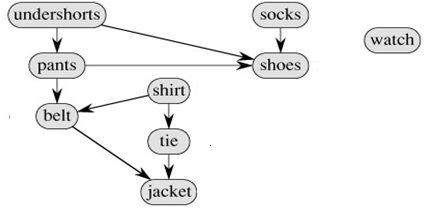
\includegraphics[width=\textwidth]{25.2}
				\label{fig:25.2}
			\end{figure}
			\end{minipage}
			& \begin{minipage}{0.6\textwidth}
				\begin{algorithm}[H]
					\caption{Topological Sort}\label{alg:topological-sort}
					\begin{algorithmic}[1]
					\Function{Topological-sort%
					\footnote{Start at any vertex, restart if necessary}%
					}{$G$}
						\State \Call{DFS}{$G$} to compute finishing times $\Call{f}{v}$ for each vertex $v$.
						\State As each vertex is finished, insert it onto the front of a linked list.
						\State \Return the linked list of vertices
					\EndFunction
					\end{algorithmic}
				\end{algorithm}
			\end{minipage}
			\\\bottomrule
		\end{tabular}
	\end{table}
	\item Why does the topological sort work?
	What is its runtime?
	\answer{We're doing a depth-first traversal, so any time there's a dependency, we access the dependency before the item that depends on it.
	$O(|V|+|E|)$.}
\end{enumerate}

\section{The Parenthesis Theorem}\label{sec:the-parenthesis-theorem}
The parenthesis theorem tells us that, for two vertices $u,v\in V$, it cannot be the case the $d[u] < d[v] < f[u] < f[v]$;
that is, the intervals $\left[ d[u], f[u] \right]$ and $\left[ d[v], f[v] \right]$ are either disjoint or nested.
This is a simple consequence of the depth-first nature of \Call{DFS}{}.
If the algorithm discovers $u$ and then discovers $v$, it cannot later back out of $u$ without backing out of $v$.

\section[Strongly Connected Components]{Strongly Connected Components (a DFS application)}\label{sec:strongly-connected-components}
A graph is said to be strongly connected if every vertex is reachable from every other vertex.
The strongly connected components of an arbitrary directed graph from a partition into subgraphs that are themselves strongly connected.
It is possible to test the strong connectivity of a graph, or to find its strongly connected components, in linear time.

\begin{algorithm}[H]
	\begin{minipage}{\textwidth}
		\caption{Strongly Connected Components}\label{alg:strongly-connected-components}
		\begin{algorithmic}[1]
		\Function{Strongly-Connected-Components}{$G$}
			\State Call \Call{DFS}{$G$} to compute finishing times $f[u]$ for each vertex $u$%
			\footnote{Restart if necessary.}
			\answer{$O(|V|+|E|)$}.
			\State Compute $G^{T}$ (the transpose of the graph)%
			\footnote{Same vertices, edges reversed.}
			\answer{$O(|E|$)}.
			\State Call \Call{DFS}{$G^{T}$}, but in the main loop of \Call{DFS}{}, consider the vertices in order of decreasing $f[u]$ (as computed in line 1)
			\answer{$O(|V|+|E|)$}.
			\State Output the vertices of each tree in the depth-first forest formed in line 3 as a separate strongly connected component.
		\EndFunction
		\end{algorithmic}
	\end{minipage}
\end{algorithm}

\begin{enumerate}[start=6]
    \item Find the strongly connected components.
	\begin{figure}[H]
		\centering
		\begin{tikzpicture}
			\begin{scope}[every node/.style={circle,thick}]
				\node (A) at (0,0) {A};
				\node (B) at (3,0) {B};
				\node (C) at (6,0) {C};
				\node (D) at (9,0) {D};
				\node (E) at (0,-3) {E};
				\node (F) at (3,-3) {F};
				\node (G) at (6,-3) {G};
				\node (H) at (9,-3) {H};
			\end{scope}

			\begin{scope}[>={Stealth[black]},
				every node/.style={fill=white,circle},
				every edge/.style={draw=black,very thick}]
				\path [->] (A) edge (B);

				\path [->] (B) edge (C);
				\path [->] (B) edge (E);
				\path [->] (B) edge (F);

				\path [->] (C) edge[bend right=7] (D);
				\path [->] (C) edge (G);

				\path [->] (D) edge[bend right=7] (C);
				\path [->] (D) edge (H);

				\path [->] (E) edge (A);
				\path [->] (E) edge (F);

				\path [->] (F) edge[bend right=7] (G);

				\path [->] (G) edge[bend right=7] (F);
				\path [->] (G) edge (H);

				\path [->] (H) edge[loop right] (H);
			\end{scope}
		\end{tikzpicture}
		\label{fig:25.3}
	\end{figure}
	\item Discuss: $G$ and $G^{T}$ will have the same strongly connected components.
	\answer{Yes, they must have the same connected components.
	They will have the same edges and cycles, they're just traveled in the opposite order.}
	\item Discuss: The component with the latest finish time vertex will have no edges in the transpose to any other component.
\end{enumerate}
%</Lecture-Activity-25>

\end{document}